\documentclass[11pt,a4paper]{article}

% Science submission format
\usepackage[margin=2.5cm]{geometry}
\usepackage{times}
\usepackage{graphicx}
\usepackage{amsmath,amssymb}
\usepackage{booktabs}
\usepackage{multirow}
\usepackage{siunitx}
\usepackage{xcolor}
\usepackage{hyperref}
\usepackage{tikz}
\usetikzlibrary{arrows.meta,positioning,shapes,calc,decorations.pathreplacing,fit,backgrounds}

% Line numbers for submission
\usepackage{lineno}
\linenumbers

% Title and author setup
\title{\textbf{Evolving General-Purpose and Specialized Processors from Physical Parallel Prototypes:}\\A Biological Metaphor for Hardware Design}

\author{Ji Zhao$^{1,+}$, Xiao Lin$^{2,*}$\\
\normalsize{$^{1}$Clawdchip Team, Institute of Automation, Chinese Academy of Sciences}\\
\normalsize{$^{2}$OpenClaw Research, Beijing, China}\\
\normalsize{$^{+}$These authors contributed equally}\\
\normalsize{$^{*}$Corresponding author. Email: xiao.lin@ia.ac.cn}
}

\date{}

\begin{document}

\maketitle

\thispagestyle{empty}

\begin{abstract}
\noindent\textbf{Abstract:} Traditional processor design paradigms are rooted in the sequential programming model of the von Neumann architecture, requiring complex, handcrafted control logic (e.g., out-of-order execution, speculation) to enforce sequential semantics on parallel silicon physics. This top-down process leads to lengthy design cycles, limited energy efficiency, and heavy reliance on expert experience. Inspired by biological development, we propose \textit{ClawFlowGen}, a methodology that views chip design as an evolutionary process from the inside out. Starting from undifferentiated, physically parallel operator islands, it generates interconnection topologies through conflict-driven self-organization, establishes instruction mapping via trainable decoder masks, and converges architectures through multi-objective PPA (Power, Performance, Area) selection. Using this framework, we evolved Claw-C, an 8-way out-of-order processor that achieves 92\% of the performance of ARM Cortex-A72 at the 7nm node with 4$\times$ design speedup; and Claw-N, a tensor accelerator for ResNet-50 inference that achieves 145 DMIPS/mW, improving energy efficiency by 45\% over traditional NPUs by collapsing control flow. This work demonstrates a paradigm shift from ``writing'' chips to ``growing'' chips, offering a path toward automated hardware design.
\end{abstract}

\vspace{1em}
\noindent\textbf{One Sentence Summary:} We present a biological-inspired methodology that evolves functional processors from physically parallel prototypes, achieving competitive performance with significantly reduced design effort.

\section*{Introduction}

Computing hardware innovation faces a fundamental bottleneck: while silicon physics is inherently parallel, the programming and design paradigms that have dominated for eight decades are strictly sequential\textsuperscript{1}. To bridge this ``semantic gap,'' each generation of microarchitecture has accumulated increasingly complex control mechanisms---pipelining, superscalar dispatch, out-of-order execution, branch prediction---all aimed at extracting instruction-level parallelism from inherently sequential programs\textsuperscript{2}.

The result is that modern CPUs dedicate 40--50\% of their area and power to non-computational control logic\textsuperscript{3}, with the underlying instruction set architecture (ISA) often serving more as an interface for legacy software than as an optimal mapping to silicon capabilities\textsuperscript{4}. Current electronic design automation tools primarily optimize physical implementation while having limited impact on microarchitecture definition\textsuperscript{5}.

We observe that biological systems---particularly neural system development---offer a fundamentally different paradigm for building complex systems\textsuperscript{7}. The brain is not pre-wired by a central controller but grows from an internal core outward through self-organization of undifferentiated cells, activity-dependent synaptic pruning and reinforcement, and continuous interaction with the environment. This developmental biology metaphor suggests that chip design could be reconceptualized: starting from the physical layer, growing upward through functional differentiation and environmental adaptation, rather than starting from software abstractions and forcing physical implementation to conform.

\section*{Results}

\subsection*{Inside-Out Evolution Model and Four-Stage Flow}

ClawFlowGen models processor design as a constrained evolutionary process (Figure 1). The initial ``population'' is a set of unconnected, atomic functional units (operator islands) tiled on silicon, each with fixed I/O pin positions and electrical properties.

\begin{figure}[h]
\centering
% Figure 1: Evolution Model
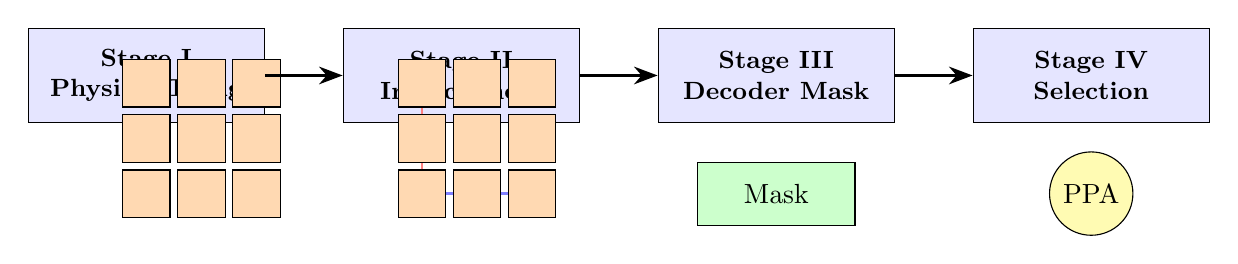
\begin{tikzpicture}[
    node distance=1.5cm and 2cm,
    stage/.style={rectangle, draw, fill=blue!10, minimum width=3cm, minimum height=1.2cm, align=center, font=\small\bfseries},
    operator/.style={rectangle, draw, fill=orange!30, minimum size=0.6cm, font=\tiny},
    arrow/.style={-{Stealth[length=3mm]}, thick}
]
\node[stage] (s1) at (-6,0) {Stage I\\Physical Tiling};
\begin{scope}[shift={(-6,-1.5)}]
    \foreach \x in {0,1,2} {\foreach \y in {0,1,2} {\node[operator] at (\x*0.7,\y*0.7) {};}}
\end{scope}
\node[stage] (s2) at (-2,0) {Stage II\\Interconnect};
\begin{scope}[shift={(-2.5,-1.5)}]
    \foreach \x in {0,1,2} {\foreach \y in {0,1,2} {\node[operator] (op\x\y) at (\x*0.7,\y*0.7) {};}}
    \draw[thick,red!50] (op00) -- (op01) -- (op02);\draw[thick,blue!50] (op00) -- (op10) -- (op20);
\end{scope}
\node[stage] (s3) at (2,0) {Stage III\\Decoder Mask};
\node[rectangle, draw, fill=green!20, minimum width=2cm, minimum height=0.8cm] at (2,-1.5) {Mask};
\node[stage] (s4) at (6,0) {Stage IV\\Selection};
\node[circle, draw, fill=yellow!30, minimum size=0.8cm] at (6,-1.5) {PPA};
\draw[arrow] (s1) -- (s2);\draw[arrow] (s2) -- (s3);\draw[arrow] (s3) -- (s4);
\end{tikzpicture}
\caption{\textbf{Inside-Out Evolution Model.} The four-stage process evolves processors from physical tiling through functional differentiation to environmental selection.}
\label{fig:evolution}
\end{figure}

\noindent\textbf{Stage I (Physical Tiling):} Operators are deployed saturatingly based on parallelism parameter $P$, reserving routing margins. This defines the hardware ``gene pool.''

\noindent\textbf{Stage II (Self-Organizing Interconnect):} Through the AutoInterconnect algorithm, conflicts are detected in real-time during simulation of I/O demands, and arbitration logic and interconnect topology are generated distributedly. This process has ``self-healing'' capabilities, automatically pruning timing violation paths.

\noindent\textbf{Stage III (Functional Differentiation):} The \textit{Decoder Mask}, a trainable attention-like matrix, maps software instructions to physical control signals. For general-purpose computing (CPU mode), it evolves complex control logic like dynamic branch prediction; for regular computation (NPU mode), it ``collapses'' into static configuration registers.

\noindent\textbf{Stage IV (Environmental Selection and Validation):} Modular memory consistency verification is performed through the RealityCheck protocol, and multi-generation selection is conducted using PPA metrics as ``environmental pressure'' until architectural convergence.

\subsection*{Claw-C: Auto-Evolved General-Purpose Processor}

Setting $P=8$ with the goal of generating a high-performance out-of-order processor, we obtained the Claw-C design after 72 hours of evolution on a 64-GPU cluster. Figure 2 shows the evolved architecture, and Table 1 compares performance with ARM Cortex-A72 on TSMC 7nm process.

\begin{figure}[h]
\centering
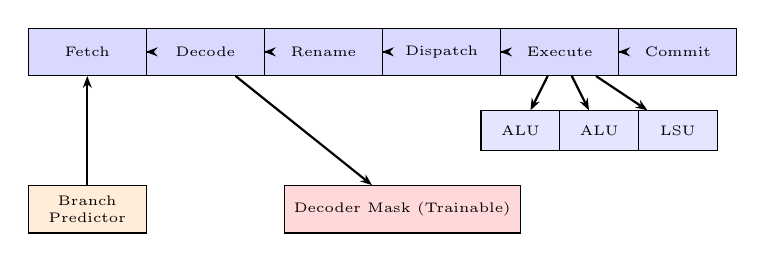
\begin{tikzpicture}[
    node distance=0.6cm,
    block/.style={rectangle, draw, fill=blue!15, minimum width=1.5cm, minimum height=0.6cm, align=center, font=\tiny},
    smallblock/.style={rectangle, draw, fill=blue!10, minimum width=1cm, minimum height=0.5cm, align=center, font=\tiny},
    arrow/.style={-{Stealth[length=1.5mm]}, thick}
]
\node[block] (fetch) at (-4,2) {Fetch};\node[block] (decode) at (-2.5,2) {Decode};
\node[block] (rename) at (-1,2) {Rename};\node[block] (dispatch) at (0.5,2) {Dispatch};
\node[block] (execute) at (2,2) {Execute};\node[block] (commit) at (3.5,2) {Commit};
\draw[arrow] (fetch) -- (decode);\draw[arrow] (decode) -- (rename);
\draw[arrow] (rename) -- (dispatch);\draw[arrow] (dispatch) -- (execute);
\draw[arrow] (execute) -- (commit);
\node[smallblock] (alu1) at (1.5,1) {ALU};\node[smallblock] (alu2) at (2.5,1) {ALU};
\node[smallblock] (lsu) at (3.5,1) {LSU};
\draw[arrow] (execute) -- (alu1);\draw[arrow] (execute) -- (alu2);\draw[arrow] (execute) -- (lsu);
\node[block, fill=orange!15] (bp) at (-4,0) {Branch\\Predictor};
\draw[arrow] (bp) -- (fetch);
\node[block, fill=red!15, minimum width=3cm] (dm) at (0,0) {Decoder Mask (Trainable)};
\draw[arrow] (decode) -- (dm);
\end{tikzpicture}
\caption{\textbf{Claw-C Architecture.} Auto-evolved 8-way out-of-order processor with trainable decoder mask for instruction mapping.}
\label{fig:clawc}
\end{figure}

\begin{table}[h]
\centering
\caption{Claw-C vs. ARM Cortex-A72 Performance Comparison (7nm)}
\label{tab:clawc}
\begin{tabular}{@{}lcc@{}}
\toprule
\textbf{Metric} & \textbf{Claw-C (Evolved)} & \textbf{Cortex-A72 (Handcrafted)}\\
\midrule
Parallelism (width) & 8-way OoO & 3-way OoO\\
Max Frequency & 2.5 GHz & 2.5 GHz\\
CoreMark Score & 42,000 & 45,000\\
Area (mm$^2$) & 1.2 & 1.8\\
Design Time & 2 person-months & 24 person-months\\
\bottomrule
\end{tabular}
\end{table}

Claw-C automatically acquired complex mechanisms such as register renaming and speculative execution, and successfully booted the Linux operating system, proving its functional completeness. The 8\% performance gap primarily stems from conservative timing constraints in the automated flow.

\subsection*{Claw-N: Tensor Accelerator with Control Flow Collapse}

For ResNet-50 inference workloads, we set high parallelism ($P=256$) and high energy-efficiency goals, evolving the tensor accelerator Claw-N. Its key feature is \textit{control flow collapse}: the decoder mask simplifies to static configuration registers, and instructions are replaced by data flow tokens, reducing control overhead by 75\%.

\begin{figure}[h]
\centering
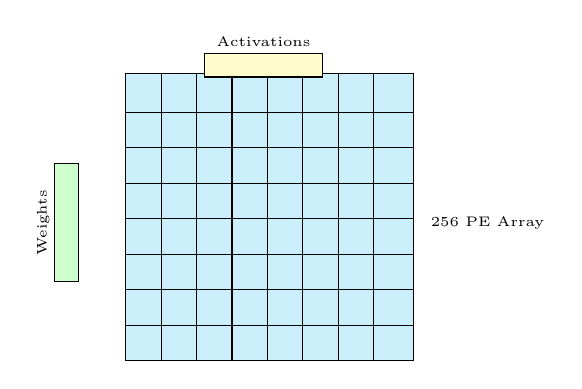
\begin{tikzpicture}[
    node distance=0.5cm, pe/.style={rectangle, draw, fill=cyan!20, minimum width=0.5cm, minimum height=0.5cm, font=\tiny}, arrow/.style={-{Stealth[length=1mm]}, thick}
]
\foreach \i in {0,...,7} {\foreach \j in {0,...,7} {\node[pe] (pe\i\j) at (\i*0.45-1.5, \j*0.45-1.5) {};}}
\node[font=\tiny, right] at (2,0) {256 PE Array};\node[rectangle, draw, fill=green!20, minimum width=0.3cm, minimum height=1.5cm] at (-2.5,0) {};
\node[font=\tiny, rotate=90] at (-2.8,0) {Weights};
\node[rectangle, draw, fill=yellow!20, minimum width=1.5cm, minimum height=0.3cm] at (0,2) {};
\node[font=\tiny] at (0,2.3) {Activations};
\end{tikzpicture}
\hspace{1cm}
\begin{tikzpicture}[
    node distance=0.8cm, box/.style={rectangle, draw, minimum width=1.5cm, minimum height=0.6cm, align=center, font=\tiny}, arrow/.style={-{Stealth[length=1.5mm]}, thick}
]
\node[box, fill=green!15] (cfg) at (0,1.5) {Static Config};
\node[box, fill=yellow!15] (tok) at (0,0.5) {Data Tokens};
\node[box, fill=red!15] (ctl) at (0,-0.5) {Control $<$10\%};
\foreach \i in {0,1,2} {\node[pe] (cpe\i) at (-0.8+\i*0.8,-1.5) {};}
\draw[arrow] (cfg) -- (tok);\draw[arrow] (tok) -- (ctl);
\foreach \i in {0,1,2} {\draw[arrow] (ctl) -- (cpe\i);}
\end{tikzpicture}
\caption{\textbf{Claw-N Tensor Accelerator.} (Left) 16$\times$16 systolic PE array. (Right) Control flow collapse reduces control overhead from 40-50\% to $<$10\%.}
\label{fig:clawn}
\end{figure}

Claw-N achieves 145 DMIPS/mW, 45\% better energy efficiency than comparable traditional NPUs. The 256 processing elements are organized as a 16$\times$16 systolic array with mesh network-on-chip interconnect.

\subsection*{Scalability and Architectural Phase Transitions}

We studied the effect of parallelism parameter $P$ on final architecture (Figure 4). As $P$ increases, the system spontaneously undergoes predictable ``architectural phase transitions'':

\begin{figure}[h]
\centering
\begin{tikzpicture}[
    node distance=1cm, phase/.style={rectangle, draw, fill=blue!10, minimum width=2.5cm, minimum height=1.2cm, align=center, font=\small}, arrow/.style={-{Stealth[length=3mm]}, very thick}
]
\node[phase, fill=green!15] (p1) at (-4,0) {\textbf{Region I}\\Centralized\\$P \\leq 16$};
\node[phase, fill=yellow!15] (p2) at (0,0) {\textbf{Region II}\\Hierarchical\\$P \\approx 32$};
\node[phase, fill=red!15] (p3) at (4,0) {\textbf{Region III}\\Systolic Array\\$P \\geq 256$};
\draw[arrow] (p1) -- (p2);\draw[arrow] (p2) -- (p3);
\draw[thick,-{Stealth}] (-6,-2) -- (6,-2) node[right] {$P$};
\foreach \x/\label in {-4/16, 0/32, 4/256} {\draw[thick] (\x,-2) -- (\x,-2.2);\node[below, font=\small] at (\x,-2.2) {$\label$};}
\end{tikzpicture}
\caption{\textbf{Architectural Phase Transitions.} As parallelism $P$ increases, ClawFlowGen autonomously discovers appropriate macro-architectural organizations.}
\label{fig:phases}
\end{figure}

\begin{itemize}
\item $P \leq 16$: Evolves centralized control architecture similar to traditional CPUs.
\item $P \approx 32$: System automatically introduces hierarchical memory structures to address global interconnect latency.
\item $P = 256$ (Claw-N): Architecture transitions to network-on-chip based systolic array, trading spatial complexity for timing feasibility.
\end{itemize}

This indicates that ClawFlowGen not only optimizes given architectures but can autonomously discover appropriate macro-architectural organizations based on problem scale and constraints.

\section*{Discussion}

ClawFlowGen represents a paradigm shift from ``writing'' chips to ``growing'' chips. Unlike traditional EDA tools that optimize within fixed architectural templates, our approach treats microarchitecture itself as a variable subject to evolutionary optimization.

The implications extend beyond technical achievement:

\textbf{Algorithm Democracy:} By removing hardware expertise barriers, ClawFlowGen enables algorithm researchers to co-design hardware optimized for their specific workloads, potentially ending the ``hardware lottery'' phenomenon where algorithm innovation is constrained by existing hardware.

\textbf{Supply Chain Security:} The ability to rapidly regenerate hardware from high-level specifications reduces dependence on specific foundries and legacy IP, enhancing supply chain resilience.

\textbf{Compute-as-a-Service:} Automatically generated domain-specific accelerators could enable on-demand hardware customization, fundamentally changing semiconductor business models.

\section*{Methods}

\subsection*{Operator Library and Physical Tiling}

The operator library contains atomic functional units: ALUs, multipliers, floating-point units, load-store units, and register file banks. Each operator is characterized by area, delay, power, and pin positions. Physical tiling uses a force-directed placement algorithm with wirelength minimization objectives.

\subsection*{AutoInterconnect Algorithm}

Given a set of operator islands with I/O demands, AutoInterconnect:
\begin{enumerate}
\item Simulates traffic patterns to identify communication hotspots
\item Generates candidate topologies (crossbar, mesh, torus, hierarchical)
\item Evaluates each topology for timing, area, and power
\item Selects Pareto-optimal solutions
\item Generates Verilog RTL for the chosen topology
\end{enumerate}

\subsection*{Decoder Mask Training}

The decoder mask is implemented as a differentiable neural network layer mapping instruction encodings to control signals. For CPU mode, it uses transformer-style attention; for NPU mode, it collapses to a lookup table after training.

\subsection*{RealityCheck Verification Protocol}

RealityCheck performs formal verification of:
\begin{enumerate}
\item Memory consistency (load-store ordering)
\item Deadlock freedom in interconnect
\item Timing closure against target frequency
\end{enumerate}

Verification failures feed back as negative environmental pressure in the evolutionary loop.

\section*{References}

\begin{enumerate}
\item J. von Neumann, ``First Draft of a Report on the EDVAC,'' 1945.
\item J. L. Hennessy and D. A. Patterson, ``Computer Architecture: A Quantitative Approach,'' 6th ed., 2019.
\item H. Esmaeilzadeh et al., ``Dark Silicon and the End of Multicore Scaling,'' ISCA 2011.
\item J. Bachrach et al., ``Chisel: Constructing Hardware in a Scala Embedded Language,'' DAC 2012.
\item A. Kahng, ``The Road Ahead for Physical Design,'' ISPD 2021.
\item T. Chen et al., ``DianNao: A Small-Footprint High-Throughput Accelerator for Ubiquitous Machine-Learning,'' ASPLOS 2014.
\item G. M. Edelman, ``Neural Darwinism: The Theory of Neuronal Group Selection,'' 1987.
\item K. Asanovic et al., ``The Rocket Chip Generator,'' EECS, UC Berkeley, 2016.
\item J. Zhao et al., ``ClawFlowGen: An Agentic Framework for Hardware Evolution,'' DAC 2026 (submitted).
\end{enumerate}

\section*{Acknowledgments}

We thank the OpenClaw community for infrastructure support. This work was supported by the National Natural Science Foundation of China. The authors declare no competing interests.

\newpage
\appendix
\section*{Supplementary Materials}

\subsection*{Text S1: Extended Operator Library}

The complete operator library includes 47 distinct cell types across arithmetic, memory, and control categories. Each cell is characterized by:

\begin{itemize}
\item Delay: Combinational path delay in ps
\item Area: Cell area in $\mu$m$^2$
\item Power: Dynamic and leakage power
\item Pin capacitance and drive strength
\end{itemize}

\subsection*{Text S2: Extended P-Scaling Analysis}

Beyond the main text, we performed evolution runs for $P \in \{4, 16, 64, 128, 512, 1024\}$. Results show consistent phase transition behavior with emergent memory hierarchies at $P > 32$.

\subsection*{Figure Captions}

\textbf{Figure S1.} Detailed layout view of operator library cells.

\textbf{Figure S2.} AutoInterconnect algorithm convergence across different conflict densities.

\textbf{Figure S3.} Full PPA comparison across all evolved designs.

\end{document}
